% This must be in the first 5 lines to tell arXiv to use pdfLaTeX, which is strongly recommended.
\pdfoutput=1
% In particular, the hyperref package requires pdfLaTeX in order to break URLs across lines.

\documentclass[11pt]{article}

% Remove the "review" option to generate the final version.
\usepackage[]{acl}
\usepackage[]{booktabs}
\usepackage{graphicx}

% Standard package includes
\usepackage{times}
\usepackage{latexsym}

% For proper rendering and hyphenation of words containing Latin characters (including in bib files)
\usepackage[T1]{fontenc}
% For Vietnamese characters
% \usepackage[T5]{fontenc}
% See https://www.latex-project.org/help/documentation/encguide.pdf for other character sets

% This assumes your files are encoded as UTF8
\usepackage[utf8]{inputenc}

% This is not strictly necessary, and may be commented out,
% but it will improve the layout of the manuscript,
% and will typically save some space.
\usepackage{microtype}

% If the title and author information does not fit in the area allocated, uncomment the following
%
%\setlength\titlebox{<dim>}
%
% and set <dim> to something 5cm or larger.

\title{Experimental Protocols: \\
\large Effect of syntactic features for multi-hop QA }

\author{Sasi Kanth Ala\\
  \texttt{sasikanth.ala@gmail.com}
}

\begin{document}

\maketitle

\section{Hypotheses} 

Choosing syntactically related examples for in-context learning and syntactical decomposition of complex question will improve performance of retrieval augmented in-context learning multi-hop QA systems.

\section{Data}

I am using HotpotQA\cite{yang-etal-2018-hotpotqa} and BeerQA\cite{qi-etal-2021-answering} to evaluate my hypothesis.

HotpotQA has 113k question-answer pairs on Wikipedia where the questions require multiple supporting passages to answer. HotpotQA is collected by crowd-sourcing where crowd workers are shown multiple supporting context documents and are asked to come up with question which require information from all the documents to answer. The questions usually fall into two categories \emph{bridge questions} and \emph{comparison questions}. To answer bridge questions one needs the passage from the previous hop to retrieve passages required for the next hop. In contrast the passages for comparison questions can be retrieved in parallel. We use train set for selecting examples for few-shot in-context learning and use dev set for evaluation.

BeerQA combines data from 1-hop SquadQA \cite{rajpurkar-etal-2016-squad}, 2-hop HotpotQA manually created 3+ hop questions. The distribution of questions is shown in 
\ref{fig:BeerQA_dist}. Unfortunately we don't have 3+ hop questions in train or dev set. Still this is a good benchmark to see if our system handle questions without prior knowledge about question complexity. We use train set for selecting examples for few-shot in-context learning and use dev set for evaluation.  

\begin{figure}[htp]
    \centering
    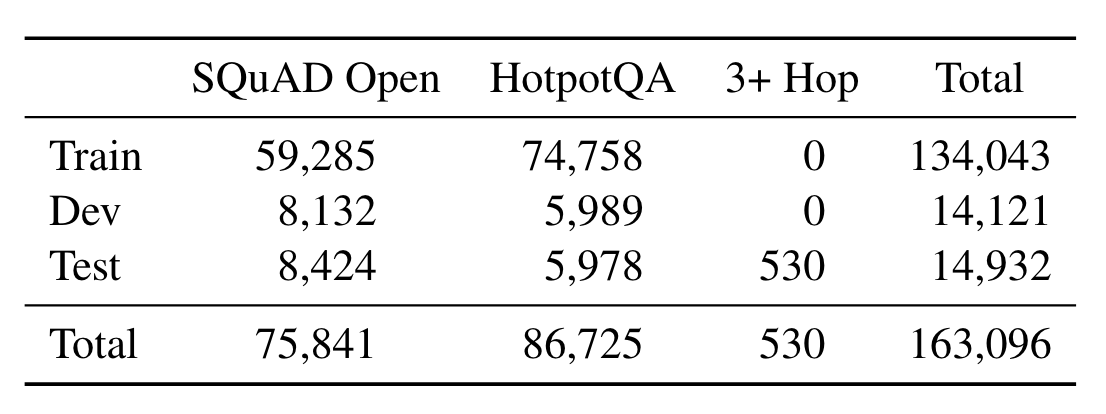
\includegraphics[width=6cm]{BeerQA-dist.png}
    \caption{Distribution of questions from sources.\cite{qi-etal-2021-answering}}
    \label{fig:BeerQA_dist}
\end{figure}

\section{Metrics} 

For evaluating the models I choose Exact Match and $F_{1}$. Exact match measures the percentage of predictions that match at last one of expected answer exactly ignoring case, punctuation and articles. $F_{1}$ (macro averaged) measures the overlap between the prediction and expected answer. $F_{1}$ score for each item is calculated by treating prediction and expected answer as bag of words and taking the maximum of $F_{1}$ across all expected answers. 

\section{Models} 

I will be using gpt-3.5-turbo as LM and ColBERTv2 with Wikipedia index.

Vanilla LM \cite{https://doi.org/10.48550/arxiv.2212.14024}: This baseline represents the few-shot in-context learning with out retriever. I will randomly sample 16 demonstrations from the train set as examples. The validation question-answers come from Wikipedia and LMs are probably trained on Wikipedia. 

multi-hop with random examples: This model uses Demonstrate Search Predict pipeline as specified in DSP paper \cite{https://doi.org/10.48550/arxiv.2212.14024}. 

multi-hop with syntactically related examples: This model will choose examples for in-context learning based on syntactic similarity to the question. For extracting syntactic information I am planning to parse the sentence using Berkeley Neural Parser\cite{kitaev-klein-2018-constituency}. For measuring similarity between parse trees I am planning to compute tree edit distance\cite{zhang_simple_1989}.

multi-hop with syntactic query decomposition: This model will use Question Decomposition Meaning Representation (QDMR)\cite{wolfson-etal-2020-break} to generate ordered list of steps that are necessary for answering a question. The ordered list encodes dependency information between the step and makes it easy to parallelize interactions between LM and RM. 

multi-hop with full syntactic features: This model combines the two previous models. It uses syntactic information for examples and question decomposition.

Table \ref{table:dev-results} shows the experimental results when finished.

\begin{table*}
\centering
\small
\vspace{2mm}
\begin{tabular}{ l @{\hspace{42pt}} cc @{\hspace{42pt}}  cc }
\toprule
& \multicolumn{2}{c@{\hspace{42pt}}}{\textbf{HotpotQA}}
& \multicolumn{2}{c@{\hspace{42pt}}}{\textbf{BeerQA}} \\
& EM & $F_{1}$ & EM & $F_{1}$ \\
\midrule
\textbf{Vanilla LM}            & -- & -- & -- & --\\
\textbf{multi-hop with random examples} & -- & -- & -- & -- \\
\midrule
\textbf{multi-hop with syntactically related examples}  & -- & -- & -- & -- \\
\textbf{multi-hop with syntactic query decomposition} & -- & -- & -- & -- \\
\midrule
\textbf{multi-hop with full syntactic features} & \textbf{--} & \textbf{--} & \textbf{--} & \textbf{--} \\
\bottomrule
\end{tabular}%
\caption{\label{table:dev-results}Development results for syntactically enhanced DSP program against baselines vanilla LM and multi-hop with random examples. It also breaks down the effect of syntactic features in example selection and complex query decomposition.}
\end{table*}

\section{General Reasoning} 

The choice of examples provided for in-context learning has big effect on its performance. Selecting examples based on semantic similarity\cite{liu-etal-2022-makes} has significant improvements for question answering. My hypothesis is choice of examples based on the question's syntactic form will give similar improvements in question answering performance.

Recently state of the art systems use LM prompting to implement many components of their systems\cite{https://doi.org/10.48550/arxiv.2210.08726}. LM models are expensive and slow. They are also stateless. Too many back and forth between LM and RM adds to the cost and query latency. It will be useful to investigate  specialized components which are faster and cheaper and which will make the whole system competitive with state of the art systems which use LM prompting extensively. Complex question answering requires decomposing the question into constituent parts which can be handled by its own specialized component instead of using LM prompting. B\textsc{reak}RC\cite{wolfson-etal-2020-break} uses high level QMDR structures for answering open-domain multi-hop questions. This semi structured decomposition has potential to be converted to database queries and included as context to LM.

\section{Summary of Progress} 

I played with sample DSP program and am able to make small changes. I was also able to get sample parsing program, tree edit distance and QMDR working. In coming days I will be joining these pieces to implement the models. 

% Entries for the entire Anthology, followed by custom entries
\bibliography{anthology,custom}

\appendix

\end{document}
